\documentclass[12pt,a4paper]{article}
\usepackage{graphicx} % Required for including images
\usepackage{xcolor}   % For custom colors in code boxes
\usepackage[utf8]{inputenc}
\usepackage{listingsutf8} % For code formatting with UTF-8 support
\lstdefinelanguage{Dockerfile}{
    morekeywords={FROM, RUN, CMD, LABEL, MAINTAINER, EXPOSE, ENV, ADD, COPY, ENTRYPOINT, VOLUME, USER, WORKDIR, ARG, ONBUILD, STOPSIGNAL, HEALTHCHECK, SHELL},
    sensitive=true,
    morecomment=[l]{#},
    morestring=[b]"
}
\usepackage{tcolorbox} % For boxed content
\usepackage[utf8]{inputenc}
\usepackage{geometry} % To set page margins
\usepackage{setspace} % For line spacing
\usepackage{setspace} % For line spacing
\geometry{a4paper, margin=1in}

% Define placeholders if not already defined
\newcommand{\mygraphicspath}{D:/SEM-5/FSDC/quantum-cloud-integration/images/ADYPU_LOGO.png}
\newcommand{\mydegree}{Bachelor of Technology}
\newcommand{\degreename}{Information Technology}
\newcommand{\vname}{Priyanshu Kumar Sharma, Neha Gaikwad, Krishna Pandey, Paavani Bargoti}
\newcommand{\mydep}{School of Engineering}
\newcommand{\vregisternumber}{2022-B-17102004A, 2022-B-01112004, 2022-B-03102004A, 2022-B-23102003}
\newcommand{\vspecialization}{Cloud Technology \& Information Security}
\newcommand{\vdate}{November, 2024}
\newcommand{\vcollege}{Ajeenkya D Y Patil University}
\newcommand{\vtitle}{Quantum Cloud Integration: Potential Impact of Quantum Computing on Cloud Storage}
\newcommand{\department}{School of Engineering}
\newcommand{\vaddresslinei}{Pune, India}
\newcommand{\vaddresslineii}{412105}    
\newcommand{\vguide}{Professor Prini Rastogi}
%\newcommand{\quantum}{D:\SEM-5\FSDC\quantum-cloud-integration\images\quantum_vs_classical.png}

% Configure listings for code formatting
\lstset{
    basicstyle=\ttfamily\footnotesize,   % Font style and size
    keywordstyle=\color{blue}\bfseries, % Keywords in blue and bold
    commentstyle=\color{green!50!black},% Comments in green
    stringstyle=\color{red},            % Strings in red
    frame=single,                       % Single-line frame around the code
    numbers=left,                       % Line numbers on the left
    numberstyle=\tiny,                  % Line number style
    breaklines=true                     % Allow line breaks
}
\begin{document}

% Title Page
\thispagestyle{empty}
\begin{center}
    % Logo of the University
    {\begin{figure}[!h]
        \centering
        \includegraphics[width=4.5cm]{\mygraphicspath}
    \end{figure}}


    {\large {\bfseries {\vtitle} \par}}


    \vspace{3\baselineskip}
    
    A PROJECT REPORT\\[0.5cm]
submitted by\\[0.5cm]
\setstretch{1.25}
    {\fontsize{14}{20}\selectfont \bfseries \vname}

{(\bfseries \vregisternumber)}
\quad\\
to
\begin{spacing}{1.25}
the \textbf{\vcollege}\\

in partial fulfillment of the requirements for the award of the Degree\\
of\\
\textbf{Bachelor of Technology}\\
in\\
\textbf{\vspecialization}
\end{spacing}
%
\quad\\[0.5cm]

\begin{spacing}{1.25}
{\fontsize{14}{20}\selectfont\bfseries \department }\\

\vaddresslinei\\
\vaddresslineii\\
{\fontsize{12}{20}\selectfont \vdate}\\
\end{spacing}
%%
\end{center}
\pagenumbering{roman}
\newpage

\begin{center}
    \includegraphics[width=4.5cm]{\mygraphicspath}\\[2cm]
    \fontsize{14}{16}\selectfont \bfseries
    DECLARATION
    \end{center}
    %
    We undersigned hereby declare that the project report 
    {\bfseries \vtitle} submitted for
    partial fulfillment of the requirements for the award of degree of \textbf{Bachelor of Technology} of
    the \textbf{Ajeenkya D Y Patil University, Pune}, is a bonafide work done by us
    under supervision of \textbf{\vguide}. This submission represents our ideas in
    our own words and where ideas or words of others have been included, we have adequately
    and accurately cited and referenced the original sources. We also declare that we have
    adhered to ethics of academic honesty and integrity and have not misrepresented or
    fabricated any data or idea or fact or source in our submission. We understand that our
    violation of the above will be a cause for disciplinary action by the institute and/or the
    University and can also evoke penal action from the sources which have thus not been
    properly cited or from whom proper permission has not been obtained. This report has
    not been previously formed the basis for the award of any degree, diploma or similar title
    of any other University. 
    
    \qquad\\[1cm]
    \begin{tabular}{llll}
    Place&:\enspace Pune\qquad  \\
    Date&: \vdate \\
    Students&: \vname
    \end{tabular}

\newpage



% Abstract
\begin{center}
    \includegraphics[width=4.5cm]{\mygraphicspath}\\[2cm]
    \fontsize{14}{16}\selectfont \bfseries
    ABSTRACT
    \end{center}

The \textbf{Quantum Cloud Integration: Potential Impact of Quantum Computing on Cloud Storage} project investigates the synergistic integration of quantum computing capabilities with classical cloud infrastructure, aiming to revolutionize storage and data processing paradigms. Quantum computing, known for its ability to tackle complex computational problems, is poised to complement the scalability and accessibility of classical cloud systems. This project highlights a hybrid architecture designed to enhance cloud storage efficiency, data security, and processing capabilities, leveraging quantum algorithms alongside traditional computational methods.  

Key components of the project include:  \\
1. \textbf{Quantum Workflow Implementation}: Quantum circuits are developed using Python and Qiskit to address specific computational tasks, such as optimizing data compression, encryption, and retrieval. The circuits interact seamlessly with classical resources, ensuring a hybrid computational workflow.  \\
2. \textbf{Dockerized Integration Framework}: The entire system is containerized using Docker, enabling modularity, portability, and simplified deployment of hybrid quantum-cloud applications. This framework bridges the gap between classical cloud resources and quantum backends.  \\
3. \textbf{Hybrid Resource Management}: The integration employs AWS for managing classical tasks, such as scalable storage and data handling, while IBM Quantum processes quantum-specific computations, such as Shor’s algorithm for factorization and Grover’s algorithm for search optimization.  \\
4. \textbf{Secure Communication Protocols}: Advanced encryption and secure socket communication ensure robust data transfer between the classical and quantum systems, mitigating potential vulnerabilities in hybrid workflows.  

The system demonstrates groundbreaking use cases, such as efficient data encryption using quantum key distribution (QKD), quantum-enhanced data indexing for cloud storage, and optimized workload distribution across hybrid resources. Challenges addressed include mitigating noise in quantum computations, managing classical-to-quantum transitions, and ensuring real-time responsiveness in hybrid tasks.  

This research underscores the transformative potential of quantum computing in reshaping cloud storage strategies. It highlights how hybrid systems can achieve unparalleled efficiency and security, paving the way for innovative cloud architectures capable of handling future data demands in a quantum era.
\newpage

% Main Sections

\begin{center}
    \includegraphics[width=4.5cm]{\mygraphicspath}\\[2cm]
    \fontsize{14}{16}\selectfont \bfseries
    \section{Introduction}
    \end{center}


    Quantum computing is poised to revolutionize various fields by solving complex problems at speeds far exceeding traditional computing. Unlike classical systems, which use binary bits, quantum computing relies on quantum bits (qubits) that can exist in multiple states simultaneously, offering exponential advantages for tasks like encryption, optimization, and data analysis. Cloud computing, on the other hand, provides scalable, accessible, and cost-efficient resources for data storage and processing. However, traditional cloud systems are reaching their limits in handling complex tasks, especially those requiring high computational power or advanced security.

    Quantum-cloud integration combines the strengths of both quantum and classical systems to address these limitations. By leveraging quantum computing for high-complexity operations such as encryption, data searching, and optimization, and using classical systems for routine tasks, this hybrid approach can enhance cloud storage and computing. Quantum algorithms, like Grover’s for faster searches and Shor’s for breaking encryption, promise to significantly improve cloud system capabilities.
    
    This research explores the implementation of quantum-cloud integration using tools like IBM Quantum for quantum algorithms, AWS for classical computing, and Docker for containerization. The goal is to create a modular, secure, and efficient system that can handle complex workloads. While challenges such as qubit coherence and system integration remain, the potential impact of this integration on industries such as healthcare, finance, and scientific research is profound. By examining both the opportunities and hurdles, this project aims to contribute to the development of future cloud systems powered by quantum computing.

\subsection{Core Concepts of Quantum-Cloud Integration}
Quantum-cloud integration is a multidisciplinary field that combines principles from quantum computing, cloud computing, and cybersecurity. Key concepts include:
\begin{itemize}
    \item \textbf{Quantum Computing}: Utilizes qubits to achieve parallelism through superposition and entanglement, enabling exponential computational speedups for specific tasks.
    \item \textbf{Cloud Computing}: Offers scalable, flexible, and cost-effective solutions for data storage and processing, essential for businesses and individual users.
    \item \textbf{Hybrid Model}: Combines quantum and classical resources, leveraging the strengths of both paradigms to optimize performance and efficiency.
\end{itemize}

\section{Quantum Computing}

Quantum computing represents a paradigm shift in computational power, leveraging the principles of quantum mechanics. In this section, we will explore the fundamental concepts of quantum computing, its comparison with traditional computing, and the tools available for quantum programming, such as Qiskit.

\subsection{Why Quantum Computing?}
Quantum computing is not just an incremental improvement over classical computing; it promises to solve problems that are currently intractable. Problems in areas like cryptography, optimization, and simulations can benefit from quantum algorithms that leverage superposition and entanglement, two key principles of quantum mechanics. These properties allow quantum computers to explore multiple solutions simultaneously, drastically reducing the time required for problem-solving in some cases.

\subsection{Quantum Computing v/s Traditional Computers}
Classical computers use binary bits (0 or 1) for computation, whereas quantum computers use quantum bits, or qubits, which can exist in multiple states at once due to superposition. This leads to exponential speedups for certain classes of problems. The comparison can be illustrated with the following figure:

\begin{figure}[h!]
    \centering
    
\includegraphics[width=0.2\textwidth]{D:\SEM-5\FSDC\quantum-cloud-integration\images\quantum_vs_classical.png}
    \caption{Comparison of Quantum and Classical Computers}
    \label{fig:quantum_vs_classical}
\end{figure}

\subsection{Qiskit: Quantum Programming Framework}
Qiskit is an open-source quantum computing software development framework developed by IBM. It allows users to write quantum algorithms, simulate quantum circuits, and run them on real quantum computers. The reasons to use Qiskit include its comprehensive set of tools, ease of integration with other platforms, and access to IBM's quantum hardware for real-world applications. Here's a simple example of a quantum circuit created using Qiskit:

\begin{tcolorbox}[title=Qiskit Example]
\begin{lstlisting}[language=Python]
from qiskit import QuantumCircuit, Aer, execute

# Create a simple quantum circuit with two qubits
qc = QuantumCircuit(2, 2)
qc.h(0)  # Apply Hadamard gate
qc.cx(0, 1)  # Apply CNOT gate
qc.measure([0, 1], [0, 1])

# Simulate the circuit
simulator = Aer.get_backend('qasm_simulator')
result = execute(qc, simulator, shots=1024).result()

# Display results
counts = result.get_counts()
print("Quantum Results:", counts)
\end{lstlisting}
\end{tcolorbox}

Qiskit allows users to design and simulate quantum algorithms without requiring advanced knowledge of quantum physics.

\subsection{Qubits v/s Traditional Bits}
Traditional computers use bits to represent information, where each bit can either be 0 or 1. On the other hand, qubits (quantum bits) are the basic unit of quantum computing, which can exist in a superposition of both 0 and 1 states simultaneously. This property, along with quantum entanglement, allows quantum computers to solve certain types of problems exponentially faster than classical computers.

Here is a graphical representation comparing bits and qubits:

\begin{figure}[h!]
    \centering
    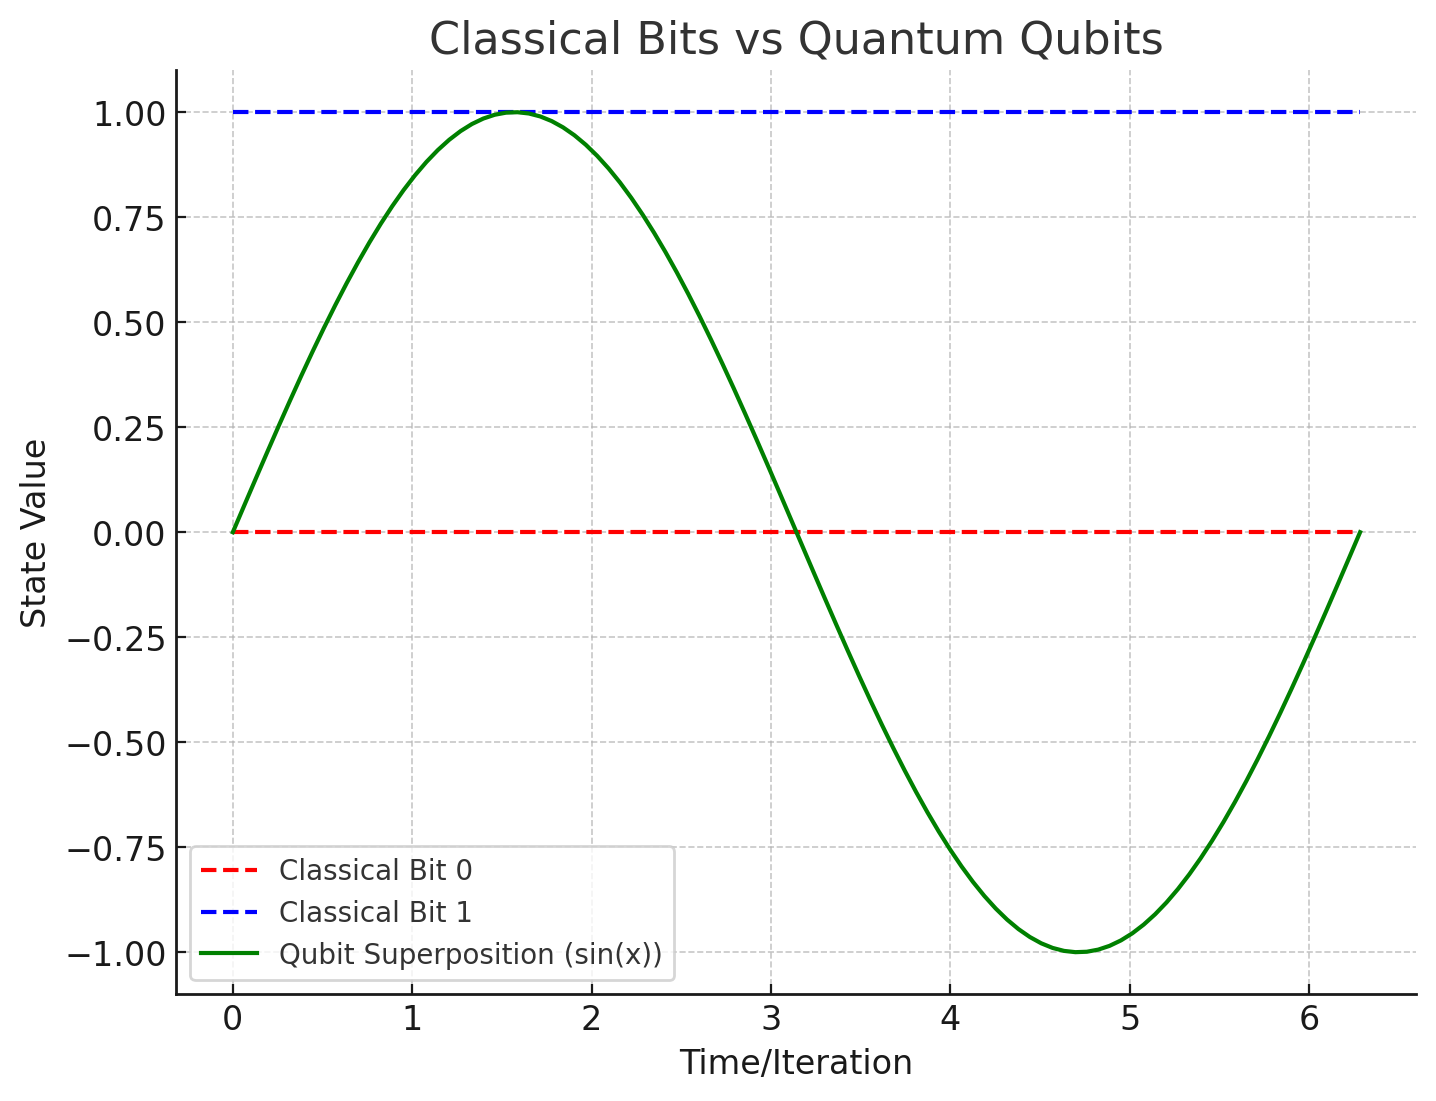
\includegraphics[width=0.8\textwidth]{qubits_vs_bits.png}
    \caption{Comparison of Qubits and Bits}
    \label{fig:qubits_vs_bits}
\end{figure}
\newpage
\section{Quantum Computing Applications}
Quantum computing has the potential to revolutionize various fields by solving complex problems that are currently unsolvable
with classical computers. Some of the key applications of quantum computing include
\begin{itemize}
\item \textbf{Cryptography:} Quantum computers can potentially break many encryption algorithms currently in
use, but they can also be used to create unbreakable encryption methods.
\item \textbf{Optimization:} Quantum computers can quickly find the optimal solution to complex
optimization problems, which can be used in fields such as logistics, finance, and energy management.
\item \textbf{Simulation:} Quantum computers can simulate complex quantum systems, which can be used in
fields such as chemistry and materials science
\item \textbf{Machine Learning:} Quantum computers can be used to speed up certain machine 
learning algorithms, which can be used in fields such as image recognition and natural language processing

\end{itemize}


\subsection{Objectives}
This paper aims to:
\begin{itemize}
   \item Develop a modular architecture to integrate quantum and classical cloud systems.
   \item Explore the application of quantum algorithms for tasks like encryption, data search, and optimization in cloud storage.
   \item Demonstrate the practical feasibility of hybrid quantum-cloud systems using real-world tools.
   \item Address technical challenges such as error rates, resource allocation, and communication protocols.
\end{itemize}

\subsection{Key Features of the Integration Framework}
The project utilizes the following tools and technologies:
\begin{itemize}
    \item \textbf{Secure Communication}: Utilizes encryption techniques for secure data transfer between quantum and classical systems.
    \item \textbf{Modular Design}: Ensures flexibility and adaptability for various applications.
    \item \textbf{Workflow Optimization}: Allocates tasks to quantum or classical systems based on computational requirements.
    \item \textbf{Fault Tolerance}: Implements mechanisms to handle quantum system errors and instability.
    
\end{itemize}

\section{Methodology}
\subsection{Framework Design}
The integration framework is built using Docker containers to manage classical cloud workloads and IBM Quantum for quantum computations. A layered approach ensures seamless interaction between quantum resources and classical systems.

\subsection{Tools and Technologies}
\begin{itemize}
    \item \textbf{Docker:} Containerization of cloud applications for easy deployment.
    \item \textbf{IBM Quantum:} Access to quantum algorithms and processing power.
    \item \textbf{AWS:} Classical cloud resources used for scalable storage and computational tasks.
    \item \textbf{Python and Qiskit:} Programming quantum algorithms and orchestration.
\end{itemize}

\subsection{Workflow}
Below is an example quantum workflow implemented in Python:

\begin{tcolorbox}[title=Quantum Circuit Example, colback=gray!5!white, colframe=blue!75!black]
\begin{lstlisting}[language=Python]
from qiskit import QuantumCircuit, Aer, execute

# Create a simple quantum circuit
qc = QuantumCircuit(2, 2)
qc.h(0)  # Apply Hadamard gate
qc.cx(0, 1)  # Apply CNOT gate
qc.measure([0, 1], [0, 1])

# Simulate the circuit on Aer simulator
simulator = Aer.get_backend('qasm_simulator')
result = execute(qc, simulator, shots=1024).result()

# Get and display results
counts = result.get_counts()
print("Quantum Results:", counts)
\end{lstlisting}
\end{tcolorbox}

\section{Implementation}
\subsection{Docker Configuration}
The Docker setup ensures an isolated environment for managing hybrid operations. Below is a snippet of the `Dockerfile`:

\begin{tcolorbox}[title=Dockerfile Example, colback=gray!5!white, colframe=blue!75!black]
\begin{lstlisting}[language=Python]
# Use an official Python runtime as the base image
FROM python:3.9-slim

# Set the working directory
WORKDIR /app

# Copy project requirements
COPY requirements.txt ./

# Install dependencies
RUN pip install --no-cache-dir -r requirements.txt

# Copy the rest of the application code
COPY . .

# Define the command to run the application
CMD ["python", "main.py"]
\end{lstlisting}
\end{tcolorbox}

% Additional Sections: Challenges, Implications, Future Scope, Conclusion, References
\end{document}
